\section{Exercise 2}

Consider the C program below:
\begin{verbnobox}[\verbarg]
#include <stdio.h>
#include <stdlib.h>
#include <string.h>
#include <stdint.h>

void vuln() {
    char str[8];

    scanf("%25s", str);
    strrev(str); // reverse the string
    if (strncmp(str, "DAVINCI:", 8) == 0) {
        printf(“%s”, str);
        return;
    }
    else
        abort();
}

void main(int argc, char** argv) {
    vuln()
}
\end{verbnobox}
\begin{enumerate}
    \item The program is affected by a typical buffer overflow. 
        Find the line affected and describe the reason. 
    \item Write an exploit for this vulnerability that must execute the following shell code, composed of 8 bytes, which opens a shell: \texttt{0x20 0x30 0x40 0x50 0x60 0x70 0x80 0x90}.
        Describe all the steps and assumptions required to successfully exploit the vulnerability. 
        Include also any assumption on how you must call and run the program: e.g., the values for the command-line arguments required to trigger the exploit correctly and/or environment variables (if any), the input provided during the execution, if multiple executions are necessary. 
    \item Make sure that you show how the exploit will appear in the process memory with respect to the stack layout right before and after the execution of the vulnerable line during the program exploitation showing:
        \begin{itemize}
            \item Direction of growth and high-low addresses.
            \item The name of each allocated variable.
            \item The content of relevant registers.
            \item The functions stack frames.
        \end{itemize}
\end{enumerate}

\subsection*{Solution}
\begin{enumerate}
    \item The buffer overflow occurs on line eight due to the buffer being sized at eight, while the program attempts to read 25 characters.
    \item The input required to exploit the vulnerability is as follows:
        \begin{verbatim}
DAVINCI:AAAA<ptr_to_shell code>\x31\x32\x33\x34\x35\x36\x37\x38
        \end{verbatim}
        However, due to the \texttt{strrev}, we need to revert the string. 
        Hence the input will be:
        \begin{verbatim}
\x38\x37\x36\x35\x34\x33\x32\x31<ptr_to_shell code_inv>AAAA:ICNIVAD
        \end{verbatim}
    \item The stack is: 
    \begin{figure}[H]
        \centering
        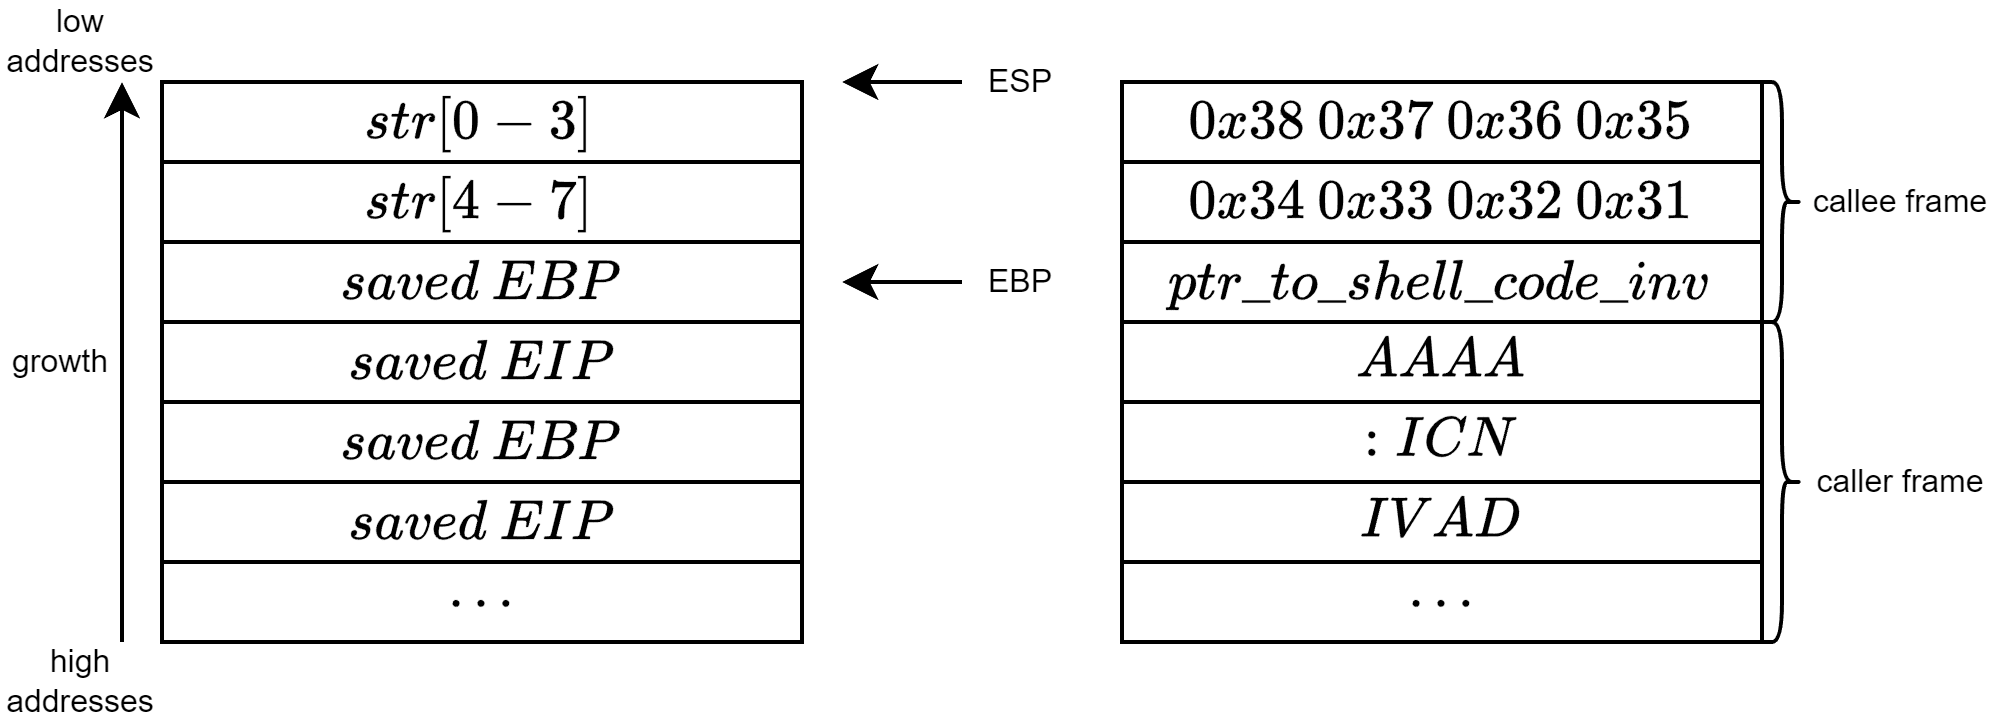
\includegraphics[width=0.85\linewidth]{images/stack2.png}
    \end{figure}
\end{enumerate}